%%%%%%%%%%%%%%%%%%%%%%%%%%%%%%%%%%%%%%%%%%%%%%%%%%%%%%%%%%%%%%%%%%%%%%
% LaTeX Example: Project Report
%
% Source: http://www.howtotex.com
%
% Feel free to distribute this example, but please keep the referral
% to howtotex.com
% Date: March 2011 
% 
%%%%%%%%%%%%%%%%%%%%%%%%%%%%%%%%%%%%%%%%%%%%%%%%%%%%%%%%%%%%%%%%%%%%%%

% Edit the title below to update the display in My Documents
%\title{Project Report}
%
%%% Preamble
\documentclass[paper=a4,12pt]{article}
\usepackage[T1]{fontenc}
\usepackage{kpfonts}
%\usepackage[fontsize=12pt]{scrextend}
\usepackage[utf8]{inputenc}
\usepackage[french]{babel}

% English language/hyphenation

\usepackage{amsmath,amsfonts,amsthm} % Math packages
%\usepackage[pdftex]{graphicx}	
\usepackage{url}
\usepackage[bottom=10em]{geometry}
\usepackage{float}
\usepackage{xcolor}
\usepackage{enumitem}
\usepackage{rotating}
\usepackage{lscape}
 


%%% Custom sectioning
%\usepackage{sectsty}
%\allsectionsfont{\normalfont\scshape}

%% Language definition package (for XML Annexe)
\usepackage{listings}
\usepackage{color}

%% Local modification of margins
%\newenvironment{changemargin}[2]{\begin{list}{}{%
%      \setlength{\topsep}{0pt}%
%      \setlength{\leftmargin}{0pt}%
%      \setlength{\rightmargin}{0pt}%
%      \setlength{\listparindent}{\parindent}%
%      \setlength{\itemindent}{\parindent}%
%      \setlength{\parsep}{0pt plus 1pt}%
%      \addtolength{\leftmargin}{#1}%
%      \addtolength{\rightmargin}{#2}%
%    }\item }{\end{list}}
%%%

%%% Custom headers/footers (fancyhdr package)
%\usepackage{fancyhdr}
%\pagestyle{fancyplain}
%\fancyhead{}											% No page header
%\fancyfoot[L]{}											% Empty 
%\fancyfoot[C]{}											% Empty
%\fancyfoot[C]{\thepage}									% Pagenumbering
%\renewcommand{\headrulewidth}{0pt}			% Remove header underlines
%\renewcommand{\footrulewidth}{0pt}				% Remove footer underlines
%\setlength{\headheight}{13.6pt}


%%% Equation and float numbering
\numberwithin{equation}{section}		% Equationnumbering: section.eq#
\numberwithin{figure}{section}			% Figurenumbering: section.fig#
\numberwithin{table}{section}				% Tablenumbering: section.tab#

%Graphics path
%\graphicspath{./Images/}

%%% Maketitle metadata
\newcommand{\horrule}[1]{\rule{\linewidth}{#1}} 	% Horizontal rule

\title{
  %\vspace{-1in} 			
  %\usefont{OT1}{bch}{b}{n}
  \horrule{1.5pt} \\[0.5cm]	
  \Huge \textbf{Projet Rain Of Music : \\ Rapport} \\ [20pt]
 % \huge TM, \\ Université d'Osaka \\ [15pt]
 	%	\vspace{1cm}  
    \LARGE Année scolaire 2015-2016 \\ 
  \horrule{1.5pt} \\[0.5cm]
  %
}

\author{						
    \LARGE \underline{Encadrants} : Jean-Michaël Celerier, \\
   					\LARGE	\hspace{5cm} Myriam De Sainte-Catherine\\			
   	\vspace{1cm} 
   	\normalfont
   	\LARGE Élèves :  Akané LEVY, Maxime PAILLASSA    
}
\date{}

%%% Begin document
\begin{document}
\graphicspath{{./imgs/}{.}}
\maketitle

\begin{figure}[H]
  \centering
\includegraphics[scale=1.2]{logo_enseirb.png}
\end{figure}

\newpage

\tableofcontents

\newpage
\normalsize


% contexte du projet
\section{Introduction}

Le but du projet Rain of music est de pouvoir scénariser un spectacle impliquant des robots et de la musique. Deux types de robots sont envisagés: des métabots (robots terrestres) et des drones (robots volant sans pilote). Ces robots doivent réaliser une chorégraphie dans un espace donné et embarquer des haut parleurs pour émettre des sons. Ce projet pluridisplinaire implique trois parties: des étudiants en arts pour la conception et l'écriture de la chorégraphie, des étudiants roboticiens pour gérer les problématiques de communication et de localisation des robots, et des étudiants en technologies multimédia (nous-mêmes) pour les sons et l'interface qui permettra aux artistes d'écrire et de simuler des chorégraphies. \\

Notre travail s'inscrit dans le début du projet (3 premiers mois) qui durera bien plus longtemps pour arriver aux objectifs finaux cités précédemment. Dans ce contexte, nous avons dû adapter nos objectifs. Ainsi, nous nous sommes fixés de réaliser un logiciel qui permettra de simuler une chorégraphie dans un espace 3D pour aider les artistes dans l'écriture d'une chorégraphie. Dans ce rapport, nous allons d'abord faire un état de l'art. Ensuite, nous allons présenter les outils que l'on a choisi pour remplir nos objectifs. Puis, nous nous intéresserons à l'architecture du logiciel et son implémentation. Enfin, nous évaluerons le logiciel en testant plusieurs scénarios différents. \\

Avant de continuer, précisons un peu les objectifs et les deux principales problématiques liées au logiciel.
Comme dit précédemment, notre travail consistera à écrire un logiciel permettant de visualiser et de simuler une chorégraphie écrite par les artistes. Cette chorégraphie est écrite grâce au logiciel i-score, qui est un séquenceur: il permet d'écrire des scénarios en programmant des évènements dans le temps. Notre travail impliquera alors deux problématiques: 
\begin{itemize}
\item la récupération des données d'i-score dans le logiciel, de manière à connaître les positions des robots.
\item l'affichage des robots dans une scène 3D, qui impliquera d'autres problématiques comme la gestion de collisions.
\end{itemize} 

\newpage

% objectifs et les motivations du projet
\input{objectifs.tex}

% ce qui existe
\section{Etat de l'art}

Dans cette partie, nous allons présenter les moyens existant nous permettant de répondre à nos objectifs. Nous verrons d'abord les moyens pour communiquer avec i-score. Ensuite, nous verrons ce qui a été fait en terme de visualisation et de simulation de performances scéniques impliquant des robots. Enfin, sera présentée l'étude des bibliothèques graphiques 3D qui nous a finalement permis de choisir l'outil pour la réalisation du projet.

\subsection{i-score}

Tout le travail réalisé devra s'interfacer avec le logiciel i-score utilisé pour écrire les chorégraphies. Pour communiquer avec un autre logiciel, i-score intègre le format OSC qui utilise le protocole UDP. Un message OSC se compose comme ceci:
\begin{lstlisting}
	<address pattern> <data type> <data>
\end{lstlisting}

L'élément \verb|<address pattern>| représente l'URL désignant la destination du message et \verb|<data type>|, une chaîne de caractères indiquant le type de données contenues dans \verb|<data>|.

Cependant, le protocole Minuit peut aussi être utilisé : ce protocole s'ajoute au protocole OSC, et permet de mieux organiser les données transmises. Les adresses OSC sont organisées dans un arbre et le logiciel pourra demander via le protocole Minuit à i-score de lui communiquer la valeur de tel ou tel paramètre. Nous verrons dans la suite de ce rapport une API qui permet de mettre en oeuvre ces fonctions pour communiquer avec i-score.

\subsection{Visualisation et simulation}

Cette partie présentera quelques articles scientifiques se rapprochant de notre projet autour des thématiques telles que la visualisation de scène 3D d'une peformance scénique et la modélisation de robot dans un espace 3D. 

Dans le domaine de visualisation de performance scénique 3D, un des objectifs est d'obtenir un rendu se rapprochant le plus possible de la réalité de façon à ce que l'on puisse avoir un aperçu réaliste de la performance conçue virtuellement. C'est dans cette optique que le logiciel de visualisation et simulation 3D StageViz\cite{StageViz} a été développé . Ce logiciel permet de visualiser en 3D en temps réel une performance scénique qui a été conçue virtuellement à l'aide d'un autre logiciel dédié à cela. Dans la forme, nous retrouvons ici, un cas très similaire à notre objectif avec la présence de visualisation mais aussi d'interopérabilité avec un outil de conception scénique.

StageViz se base sur trois éléments principaux que l'on doit aussi retrouver dans notre projet : les objets 3D, la manipulation de la scène et la chronologie. Dans le cadre de notre projet, les objets 3D représenteront les robots et la scène pourra être visionner sous tous les angles grâce à une camera mobile. En ce qui concerne la composante temporelle, elle sera gérée au niveau d'i-score qui nous envoie les données sur les robots au fur et à mesure. 

Une grande différence entre StageViz et notre projet réside dans l'utilisation du rendu 3D. StageViz serait un outil pour une simulation réaliste pour visionner les différents états des objets dans la scène au cours de la performance. Notre but serait de visualiser l'évolution des positions des robots dans la scène pour aider l'écriture de la chorégraphie. L'idée est donc d'avoir un rendu permettant une vision simplifiée et globale de la chorégraphie avec tous les robots.

Dans le domaine de performance par les robots, une équipe de recherche a étudié la modélisation des différents mouvements d'un robot dans le but de visualiser une performance \cite{robotArt}. Le robot n'est pas considéré en tant qu'un seul objet avec une position mais comme un ensemble de composants possédant des paramètres (degré de liberté) et organisés hiérarchiquement. Ainsi lorsqu'un mouvement est exécuté au niveau d'une composante, il est appliqué à toutes ses composantes filles.

Pour notre logiciel, la possibilité de modéliser les différents mouvements d'un robot est bien sûr intéressante mais ne représente pas une priorité : en effet, la chorégraphie comptera plus d'une dizaine de robots et notre simulation mettra plus en avant une vue d'ensemble de la chorégraphie que le mouvement de chaque robot. Cet article indique donc une possibilité de fonctionnalités à implémenter dans notre logiciel.

\subsection{Bibliothèques graphiques}
Dans cette partie, nous allons présenter différentes bibliothèques graphiques 3D que nous pourrions utiliser: OpenSceneGraph, openFrameworks, Ogre, Blender, Unity, Qt3D, Babylon.js et Three.js. Toutes ces bibliothèques sont basées sur OpenGL (ou WebGL) et la raison pour laquelle nous préférions utiliser une de ces bibliothèques et non OpenGL réside dans l'hypothèse que le temps de réalisation nécessitée serait plus important avec OpenGL pour un résultat équivalent.


Toutes les bibliothèques citées ci-dessus sont déployables sur pratiquement toutes les plateformes (y compris smartphones et tablettes). Celles qui sont orientées objets permettent d'avoir une programmation plus haut niveau tout en profitant des performances d'OpenGL. Elles intègrent également des packages additionnels permettant d'avoir des rendus 3D plus poussés. Les deux biblithèques Babylon.js et Three.js se déploient sur navigateur via JavaScript et utilisent WebGL.


\subsubsection{openFrameworks}

openFrameworks est open source, sous license MIT (compatible GPL), basée sur du C++ et OpenGL. Elle permet également d'intégrer et d'utiliser d'autres bibliothèques comme OpenCV par exemple, qui pourrait être utilisée pour de la gestion de trajectoires et de collisions, et de gérer des flux audio, ce qui peut s'avérer utile dans l'optique d'embarquer des haut parleurs sur les robots pour générer des sons. 

De plus, une des lignes directrices de ce projet actif est la simplicité: la bibliothèque est faite de manière à pouvoir être utilisée avec un minimum de connaissances, et propose des tutoriaux sur des bases comme l'OpenGL ou la programmation orientée objet. Ceci est un atout dans notre contexte puisque nous avons peu de temps pour implémenter le projet qui sera ensuite plus facile à reprendre par d'autres personnes.

\subsubsection{OpenSceneGraph}

OpenSceneGraph est une bibliothèque 3D open source distribuée sous la license OSGPL (OpenSceneGraph Public License) basée sur la license LGPL. Elle est écrite en C++ et en OpenGL et est utilisée dans de nombreux domaines: réalité virtuelle, jeux vidéos, visualisation scientifique et simulation. 

Le monde 3D virtuel est représenté par un graphe dont les noeuds sont logiquement et spatialement organisés. Cette vision pourrait nous nécessiter un temps d'adaptation et dans le cadre de ce projet destiné à être repris par d'autres personnes, cela pourrait s'avérer être problématique. De plus, la communauté OpenSceneGraph ne semble pas très active, ce qui représente un désavantage lors de la phase d'implémentation.

\subsubsection{Ogre}

Ogre est encore une biliothèque open source, sous license MIT, écrite en C++ et OpenGL. Elle est beaucoup utilisée pour réaliser des jeux vidéos et faire des modélisations 3D de personnages. Dans notre cas, nous n'avons pas besoin d'aller si loin au niveau du rendu 3D. L'objectif est plus d'avoir un rendu clair et fidèle à la chorégraphie, la modélisation des objets 3D importe peu. 


\subsubsection{Qt3D}

Qt est un framework utilisé pour faire des interfaces graphiques. Qt est open source, écrit en C++ sous license GNU GPL ou LGPL selon les versions. Le module Qt3D permet de faire de la modélisation 3D. Cependant, ce module est encore en cours de développement. L'utiliser serait donc prendre le risque de devoir changer plus tard du code déjà écrit, ce qui peut être problématique surtout après que le projet soit repris par d'autres personnes. 

\subsubsection{Blender et Unity}

Blender et Unity sont deux logiciels de modélisation et d'animation 3D écrits en C, C++ et Python (Blender) et C\# (Unity). Blender est open source alors que Unity ne l'est pas, même si des licenses gratuites sont proposées. Un des avantages de ces logiciels est leur communauté qui est très active.

De la même manière qu'avec Ogre, ces logiciels se dirigent plus vers du rendu 3D pour des jeux vidéos et de la modélisation 3D alors que notre objectif premier est la visualisation. 

De plus, ces logiciels proposent des interfaces pour créer facilement des objets 3D ou des textures par exemple mais ce qui nous intéresse plus est la gestion de ces objets. Par ailleurs, nous préférions un développement du projet sous forme de programmation à une réalisation du projet utilisant les interfaces graphiques de ces logiciels.

\subsubsection{Babylon.js et Three.js}

Babylon.js et Three.js sont des bibliothèques en JavaScript qui utilisent WebGL pour avoir un rendu visuel dans le navigateur. Les deux sont open source, mais Three.js est sous license MIT alors que Babylon.js est sous une license Apache, qui cherche encore à être compatible avec la license GPL. L'avantage de ces bibliothèques est que seul un navigateur est nécessaire pour visualiser la scène, ce qui les rend très accessible. Cependant, plus le projet avancera et se complexifiera (possibilité de modifier la chorégraphie par exemple), plus il nous semble compliqué d'utiliser du JavaScript qui n'est pas adapté aux projets complexes.








% choix d'outils
  % openframeworks
  % OSSIA API / Jamoma
\section{Outils utilisés}

Dans cette partie, nous allons présenter les outils que l'on a utilisé pour réaliser simulationRainOfMusic. Nous présenterons d'abord l'API d'OSSIA qui a été utilisée pour la communication avec i-score. Ensuite, nous représenterons les bibliothèques graphiques 3D évoquées précédemment et expliquerons le choix que nous avons fait.

\subsection{L'API d'OSSIA}

OSSIA est l'acronyme pour Open Scenario System for Interactive Application. Comme son nom l'indique, c'est un projet de développement d'outils logiciels de scénarisation pour des applications intéractives. Le logiciel i-score a été écrit dans le cadre de ce projet. 

Dans simulationRainOfMusic, nous utilisons l'API implémentée dans le projet OSSIA pour pouvoir communiquer avec i-score via le protocole minuit. L'API nous permet de réaliser les principales fonctions dont nous avons besoin: envoyer des données vers i-score et récupérer des données d'i-score depuis simulationRainOfMusic.  Minuit fonctionne en organisant les données sous forme d'arbre. Dans simulationRainOfMusic, on va créer des robots qui ont certains attributs et l'API va nous permettre de créer les noeuds de l'arbre correspondant aux robots et à leurs attributs et de les envoyer à i-score. L'API va également nous permettre d'écouter les attributs des robots pour les actualiser dans simulationRainOfMusic et permettre l'affichage des robots. 

Des exemples simples de fonctionnement sont disponibles dans les exemples Minuit\_publication et Minuit\_Exploration de la documentation de l'API. Un arbre est publié et partagé par Minuit\_publication et Minuit\_exploration explore cet arbre et renvoie sa structure.

\subsection{Bibliothèques graphiques 3D}

Dans cette partie, un bilan de l'étude des différents biblitohèques sera présentée sous forme de tableau avec cinq critères jugés importants dans le choix de la biliothèque. Parmi ces cinq, ne seront pas présentées ceux élémentaires telles que la présence d'un moteur 3D complet, l'aspect multi-plateforme, pour lesquelles il semble évident que toutes les bibliothèques citées jusque là les remplissent.

Un des critères qui nous a paru essentiel dans le développement du logiciel est l'auto-suffisance de la bibliothèque. C'est-à-dire un choix de possibilité assez large proposé dans la bibliothèque de base pour éviter l'utilisation de plusieurs outils annexes. Par exemple, nous avons vu pour Babylon.js qu'il faudrait l'utilisation d'autres outils (Node.js ?) pour pouvoir réaliser la réception de messages UDP. 

Un critère moins important dans une première partie du développement mais qui serait nécessaire par la suite est la présence d'un moteur physique. En effet, il serait intéressant d'avoir des fonctionnalités pour la détection de collisions, permettant ainsi d'alerter l'artiste lors de la conception de la chorégraphie.

Plus généralement, certains critères choisis pour ce bilan ont été réfléchi en vue de l'interopérabilité de notre logiciel avec i-score : l'aspect open source (notamment license GPL) et le langage utilsé. En effet, il nous semblait plus pertinant de respecter une unicité de langage avec i-score, et donc choisir le C++. 
D'autres critères ont été pensé dans l'optique de la maintenabilité, notamment la facilité à prendre en main les différentes fonctionnalités de la bibliothèque, la stabilité des versions proposées, la présence d'une communauté active (tant au niveau développeurs qu'utilisateurs).



Les critères qui ont donc été choisi pour ce bilan sont : 
\begin{itemize}
\item open source et notamment license GPL comme le logiciel i-score 
\item détection de collisions (moteur physique)
\item auto-suffisant (facilité d'utilisation d'UDP)
\item unicité du langage avec i-score (C++)
\item facilité à prendre en main
\item maintenabilité (bonne communauté active)
\end{itemize} 
 

\newpage
\begin{landscape}
\hspace{-4.5cm} 
\begin{tabular}{l|c|c|c|c|c|c|c|c}
Bibliothèque & open source & moteur physique & auto-suffisant & langage & prise en main & maintenabilité & stabilité & communauté active\\
\hline
openFrameworks & Oui & Oui & Oui & C++ & Bonne & Oui & Oui & Fort\\
OpenSceneGraph & Oui & Oui & Oui & C++ & Moyenne & Oui & Oui & Moyen\\ 
OGRE & Oui & Oui & Oui & C++ & Moyenne & Oui & Oui & Fort\\
Qt3D & Oui & Oui & Oui & C++ & Moyenne & Oui & Non & Faible\\
Unity & Non & Oui & Oui & C\# & Bonne & Oui & Oui & Fort\\
Babylon.js  & Non & Oui & Oui & JavaScript & Bonne & Oui & Oui & Moyen/Fort
\end{tabular}
\end{landscape}

Finalement, presque toutes les bibliothèques conviennent en terme de performances et de fonctionnalités. Le choix s'est donc porté sur les derniers critères (prise en main, maintenabilité, stabilité et communauté) qui s'avèrent être aussi importants dans le cadre de notre projet. Ainsi, nous avons choisi d'utiliser openFrameworks, qui semble être la meilleure par rapport à l'ensemble des critères.  


% architecture et implémentation
  % archi
  % implementation
    % visualisation
    % communication
    % simulation
\section{Architecture et implémentation du logiciel}

\subsection{Architecture}

\subsection{Implémentation}

\subsubsection{Visualisation}

\subsubsection{Communication}

\subsubsection{Simulation}

% évaluation et validation
\section{Évaluation du projet}

Dans cette partie, nous allons évaluer le projet. Nous évaluerons d'abord le logiciel dans ses trois principales parties. Ensuite, nous verrons son utilisabilité pour les artistes et l'écriture de la chorégraphie. Enfin, d'une manière plus générale, nous aborderons la gestion du projet. 

\subsection{Validation du logiciel} %validation des fonctionnalités du logiciel 

Dans cette partie, nous vérifions que les principales fonctionnalités sont correctes. On s'intéressera aux trois parties du logiciel séparément: la visualisation, la communication et la simulation. 

\subsubsection{Visualisation}

Concernant la visualisation, les trois critères importants pour évaluer cette partie sont : la fluidité des mouvements, la maniabilité de l'environnement 3D et l'ergonomie de l'interface utilisateur. 

La fluidité des images est assurée par un nombre d'images par seconde fixé à 60 fps, ce qui permet d'avoir un rendu agréable et fluide. La chorégraphie imaginée par les étudiants compterait 10 robots metabot, et dans ces conditions le nombre d'images par seconde est toujours 60 fps : l'image est fluide et l'interface réagit instantanément (pour un utilisateur, la différence de vitesse ne se sent pas entre 1 et 10 robots).
Nous avons testé pour 100 robots, le lancement de l'application prend du temps et le nombre d'images par seconde est divisé par 2, on a donc 30 fps ce qui reste correct pour une visualisation. 

La maniabilité de l'environnement 3D repose principalement sur les déplacements de la caméra de type rotation et zoom. Les deux sont rendus possibles grâce à la classe \verb|EasyCam| d'openFrameworks qui permet d'avoir une caméra simple munie des fonctionnalités usuelles (rotation, zoom, calibrage à l'initialisation automatique par rapport au milieu de la scène). Ainsi, l'utilisateur retrouve un environnement 3D usuel.

Nous avons essayé de penser à l'ergonomie, en rajoutant des menus déroulant pour chaque robot dans l'interface, ce qui permet d'éviter que le panel n'envahisse tout l'écran. De plus, un message d'aide est affiché au lancement du logiciel, il explique les touches à utiliser pour afficher des axes ou la graduation en plus, et aussi pour cacher ce message d'aide.
De même l'affichage de message de sélection permet à l'utilisateur d'identifier facilement les robots, sans qu'il ait à regarder le panel des positions.

Par ailleurs, pour alerter l'utilisateur de collision, nous avons choisi d'afficher un cercle rouge à l'emplacement du cercle mais aussi d'afficher un message informatif en haut de l'écran. Cela permet d'assurer que cet événement soit bien visible. En effet, si l'utilisateur zoom sur d'autres robots, il risque de ne pas voir le cercle rouge, alors que le message est toujours affiché au même endroit puisqu'il ne dépend pas de la scène 3D. Le cercle rouge permet tout comme le message de sélection, d'identifier plus facilement l'emplacement de la collision.

\subsubsection{Communication réseau}

Au niveau de la communication, nous avons comparé la fréquence d'appel à la méthode \verb|update| de la classe \verb|ofApp| de mise à jour de la scène par rapport à la fréquence d'i-score. En effet, on pourrait avoir des problèmes de temps si la méthode \verb|update| était appelée à une fréquence moins élevée que le tic d'i-score car on pourrait avoir des données d'i-score qui ne seraient pas mises à jour dans simulationRainOfmusic : par exemple si la fonction \verb|update| est appelée toutes les 50 ms et que le tic d'i-score est de 20 ms. 

En réalité, la méthode \verb|update| est appelée toute les 16 ms et le tic d'i-score est de 40 ms par défaut. Ainsi, les données utilisées par simulationRainOfMusic sont toujours synchronisées par rapport à celles d'i-score. On pourrait même imaginer une petite diminution de la fréquence d'appel à \verb|update| pour soulager l'utilisation de ressources, notamment lors d'une représentation avec beaucoup de robots. 

Par ailleurs, comme simulationRainOfMusic a un taux de rafraîchissement plus élevé, certaines données ne sont pas mises à jour dans i-score, notamment lorsque l'utilisateur modifie des paramètres à l'aide d'un slider via l'interface. Cependant le logiciel i-score possède la possibilité de faire des interpolations, ainsi il n'est pas nécessaire qu'i-score reçoive toutes les modifications au niveau de l'interface de simulationRainOfMusic. 

\subsubsection{Simulation}

A propos de la simulation du logiciel, plusieurs aspects peuvent être vérifiés.

D'abord, l'échelle spatio-temporelle : chaque graduation représente un mètre et si un metabot reçoit les commandes indiquant des mouvements de vitesse $dx=100 mm.s^{-1}$ ou $dy=100 mm.s^{-1}$, celui-ci avance bien d'une graduation toutes les dix secondes.

Ensuite, la consommation de la batterie des robots se fait bien linéairement en fonction de la distance parcourue par le robot en question. Si on fait parcourir dix mètres à un robot, une même quantité de batterie est consommée sur chaque mètre. A l'arrêt, les robots ne consomment pas. Des expérimentations pourraient être faites pour avoir un modèle de consommation plus réaliste. Par exemple, on pourrait s'intéresser à la consommation à l'arrêt ou selon la vitesse et la fréquence de pas quand le metabot est en mouvement.

Enfin, pour la perte de paquet, on peut compter le nombre de paquets perdus et reçus et retrouver le pourcentage de perte correspondant. Pour que celui-ci soit réaliste, on pourrait faire des expérimentations pour l'évaluer mais le protocole de communication n'est pas encore décidé définitivement (Bluetooth ou XBee). 

\subsection{Confrontation du logiciel avec les artistes}

Dans le cadre d'une rencontre avec les artistes, nous avons pu commencer à écrire la chorégraphie qu'ils avaient conçu. Ainsi les deux figures suivantes présentent un des tableaux que les artistes avaient conçu (figure \ref{chore}), et la visusalisation avec notre logiciel (figure \ref{reveil}). La chorégraphie dans son ensemble est en Annexe sous forme de storyboard. 

Une partie que nous avions commencé à travailler ensemble concernait un des derniers tableaux de la chorégraphie : la ronde que les robots font tout en s'arrêtant quelque fois pour tourner sur eux-mêmes. Pour cela, il fallait définir deux vitesses angulaires et un vecteur de déplacement pour que le robot puisse tourner en cercle et sur lui-même. La réalisation de ce mouvement s'est faite avec i-score et notre interface permettait de vérifier rapidement le résultat.

Les artistes semblaient être intéressés par la visualisation que nous proposions. Par ailleurs, cette session de travail avec eux nous a permis de tester à nouveau notre logiciel, de régler certains bugs liés à des fonctionnalités récentes et donc d'améliorer notre travail. 

Ce fut donc une session nécessaire pour le développement et l'évaluation de notre logiciel. Un aspect qui n'a pas pu être abordé et qui aurait été intéressant pour la suite du projet : lancer une chorégraphie avec i-score, et vérifier les différences entre la réalité, les véritables mouvements des robots qui exécutent les commandes d'i-score, et la simulation, la chorégraphie réalisée dans la scène virtuelle de notre logiciel.

%\hspace*{-12cm}
\begin{figure}[H]
\centering
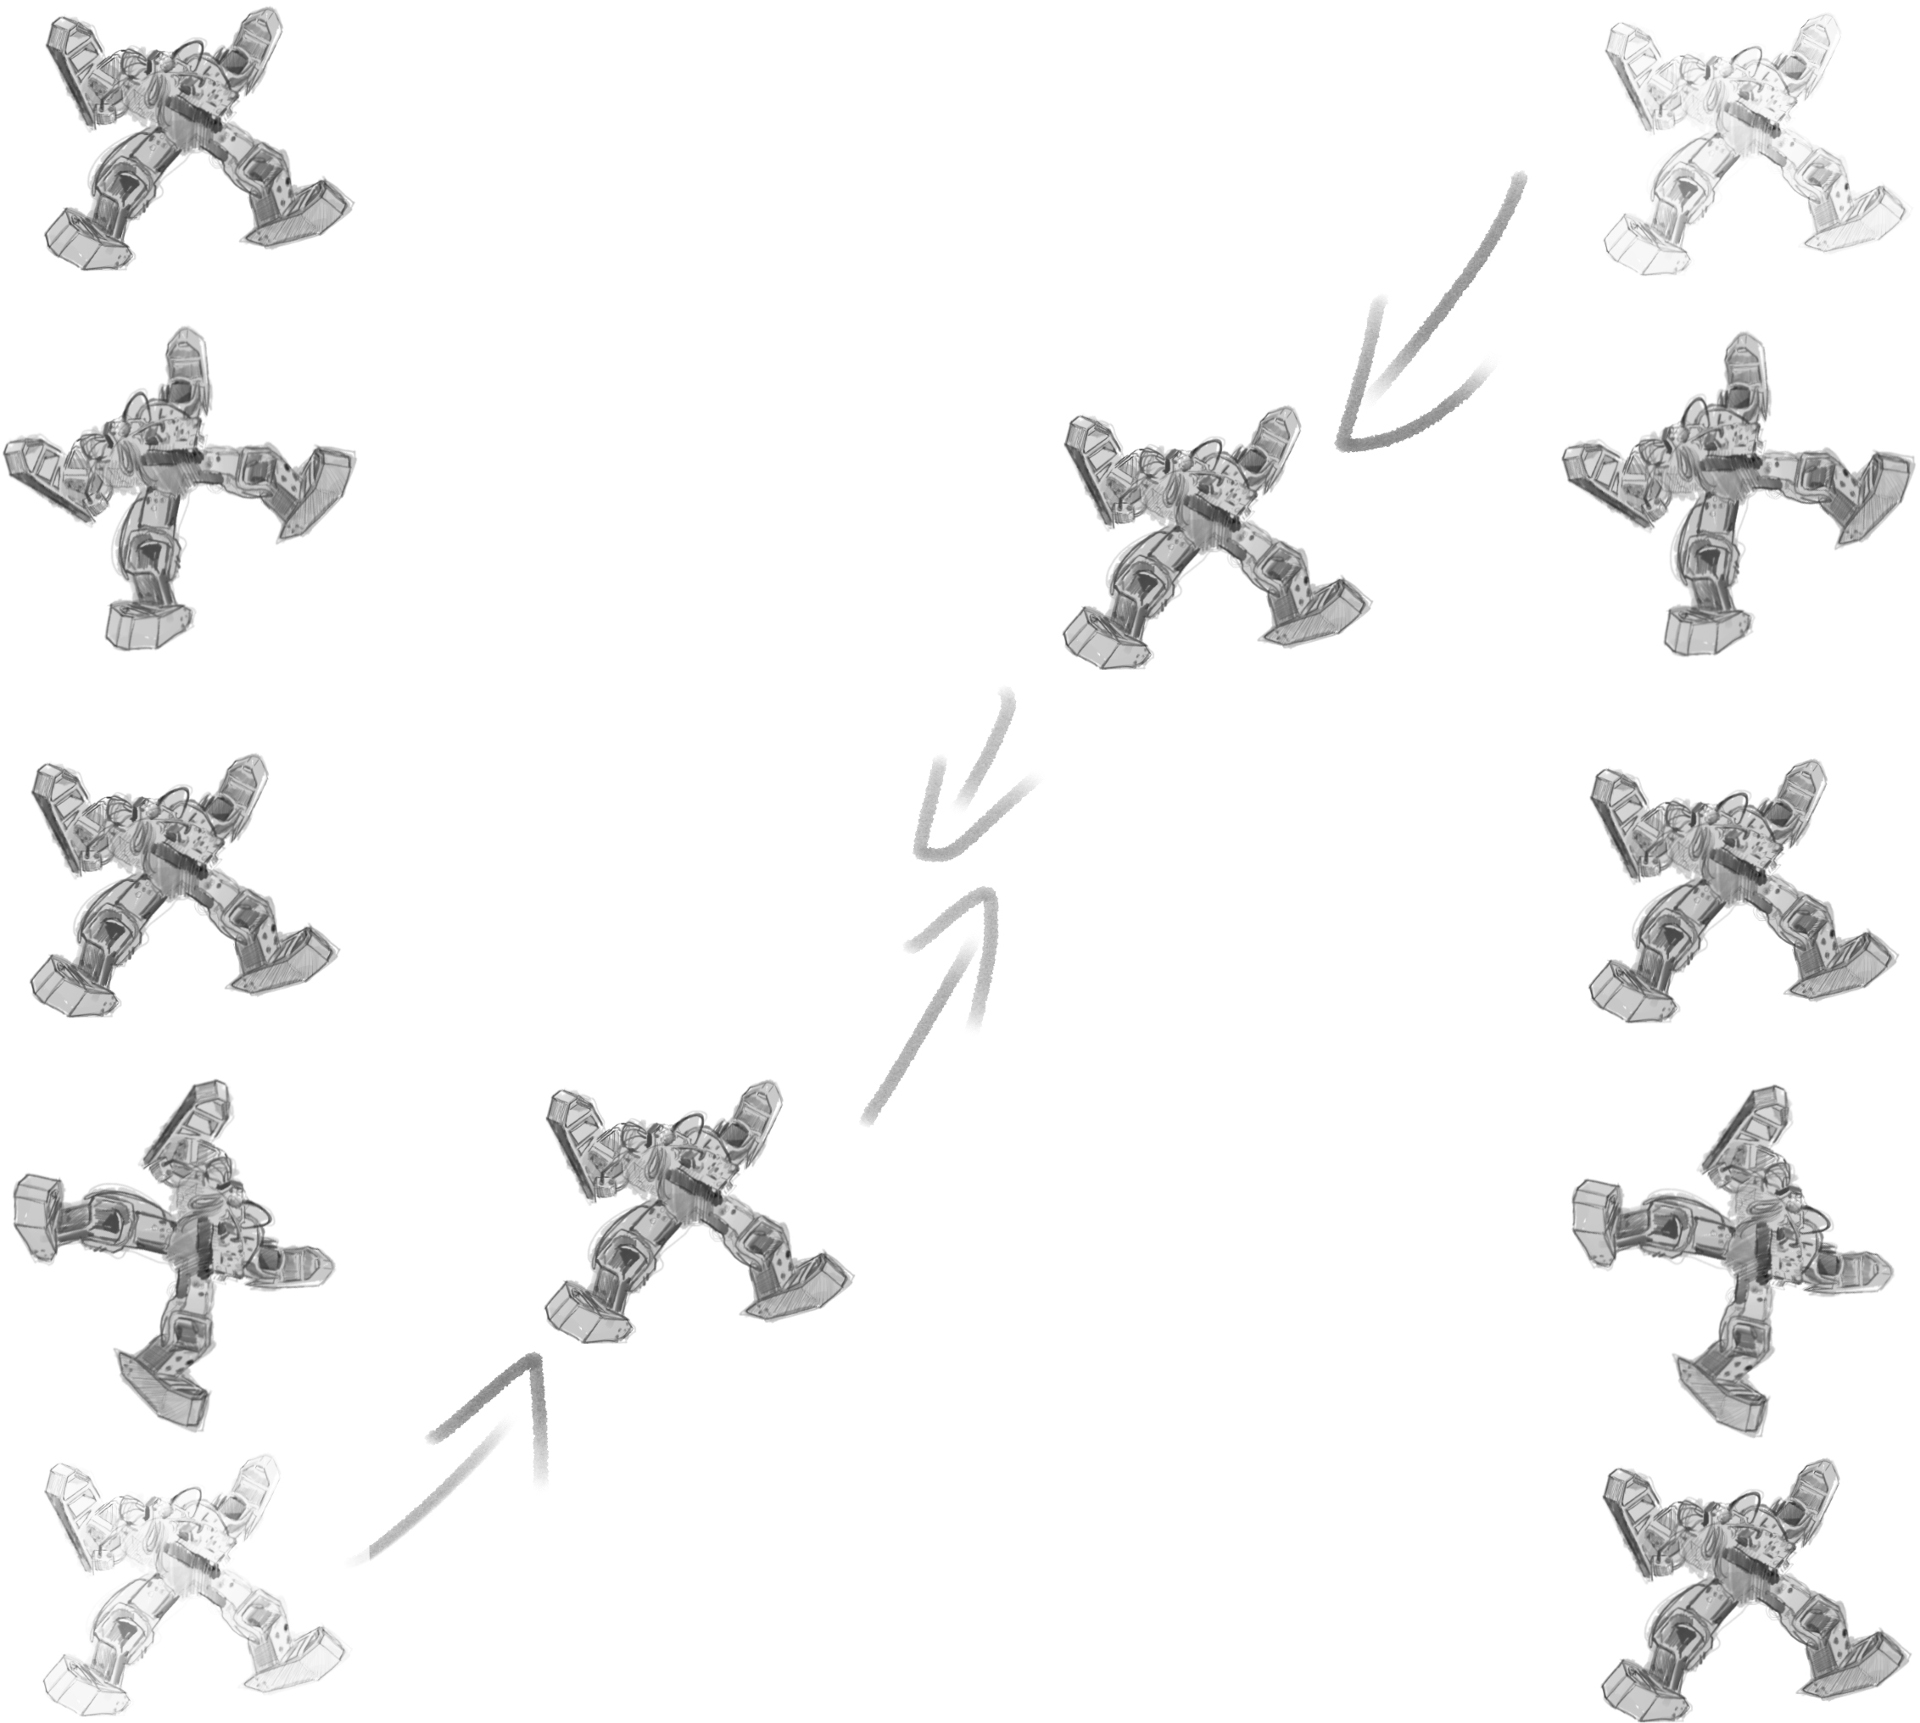
\includegraphics[scale=1.0]{reveildessin}
\caption{Dessin original des étudiants d'art de Bilbao}
\label{chore}
\end{figure}


\begin{figure} [H]
\centering
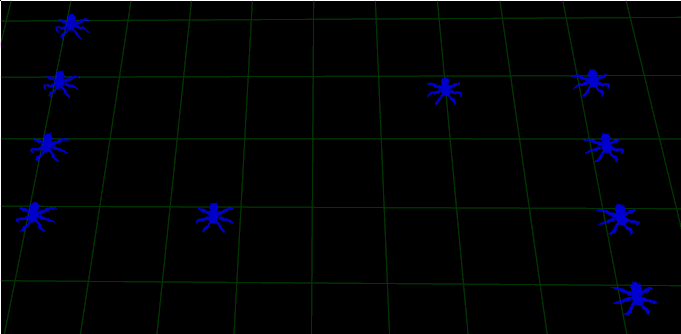
\includegraphics[scale=0.9]{reveil2}
\caption{Simulation du tableau avec notre interface simulationRainOfMusic}
\label{reveil}
\end{figure}


\subsection{Gestion du projet: calendrier et difficultés}

Dans cette partie, nous verrons la gestion du projet par rapport au calendrier que nous nous étions fixé. Puis nous verrons les difficultés que nous avons rencontrées. Un calendrier bilan est représenté sur la figure suivante \ref{cal}:

\begin{figure}[H]
  \begin{center}
  	\includegraphics[scale=0.7]{imgs/calendrierbis.png}
  	\caption{Calendrier bilan. En noir ce qui était prévu. En rouge ce qui était prévu mais qui n'a pas été fait. En vert ce qui a été fait mais qui n'était pas prévu}
  	\label{cal}
  \end{center}
\end{figure}

On remarque que finalement le calendrier de départ a subi beaucoup de changements. D'une part, la partie de simulation des mouvements des drones a été abandonnée car le projet s'est focalisé sur la mise en place des metabots en premier. D'autre part, la partie communication ne s'est pas déroulée comme prévu. L'intégration de la communication avec i-score dans simulationRainOfMusic (intégration de l'API d'OSSIA dans simulationRainOfMusic) nous a pris du temps. Une fois l'API en place, la communication avec i-score s'est établie assez facilement. 

Ensuite, l'ajout des panels dans l'interface de simulationRainOfMusic et la possibilité de modifier les paramètres des robots via ces panels ont posé deux problèmes: la communication entre l'interface et le reste du logiciel, qui a donné lieu à la classe \verb|Parameter| et la synchronisation entre l'interface de simulationRainOfMusic et i-score. En effet, pour ce dernier, une boucle infinie peut facilement apparaître comme vu précédemment car les listener vers i-score et vers l'interface de simulationRainOfMusic déclenchent automatiquement la mise à jour des valeurs qu'ils écoutent. 



% conclusion
\section{Conclusion}
\subsection{Bilan}


\subsection{Apport de notre travail dans le projet RainOfMusic}
ce que notre travail a finalement apporté au projet dans globalité (possibilité de simuler mais aussi d'écrie la chorégraphie avec notre logiciel : un plus qui n'avait pas vraiment explicité dans les besoins au début)

\subsection{Améliorations envisageables}
initialisation de la scène (ajuster les dimensions et les échelles) dans l'interface utilisateur et non dans le code 

rajout de façon dynamique des robots via l'interface utilisateur (et non en dur comme dans l'implémentation actuelle)

côté simulation, mouvements des drones et pannes probables ..?


%\subsection{Apport personnel}
%peut être écrire un paragraphe chacun avec ce que ça nous apportait ..?

  \newpage

  \bibliographystyle{plain}
  \bibliography{bibli.bib}
  \newpage

  \appendix
  \part*{Annexes}
  %\section{Manuel d'utilisation}
%manuel d'utilisation pour artiste (léger, avec i-score create device) et pour développeur () 

\section{Chorégraphie}
Voici la chorégraphie sous forme de storyboard conçue par les étudiants d'Art de l'université de Bilbao. On peut distinguer que le spectacle est divisé en plusieurs parties, l'image du storyboard correspondant est indiqué entre parenthèses : le réveil (1), la rencontre (2), la danse (3-10), la percussion avec un rythme particulier engendré par les pattes des robots (11-12), la dernière ronde (13), le retrait (14-18).

\hspace*{-2cm}
%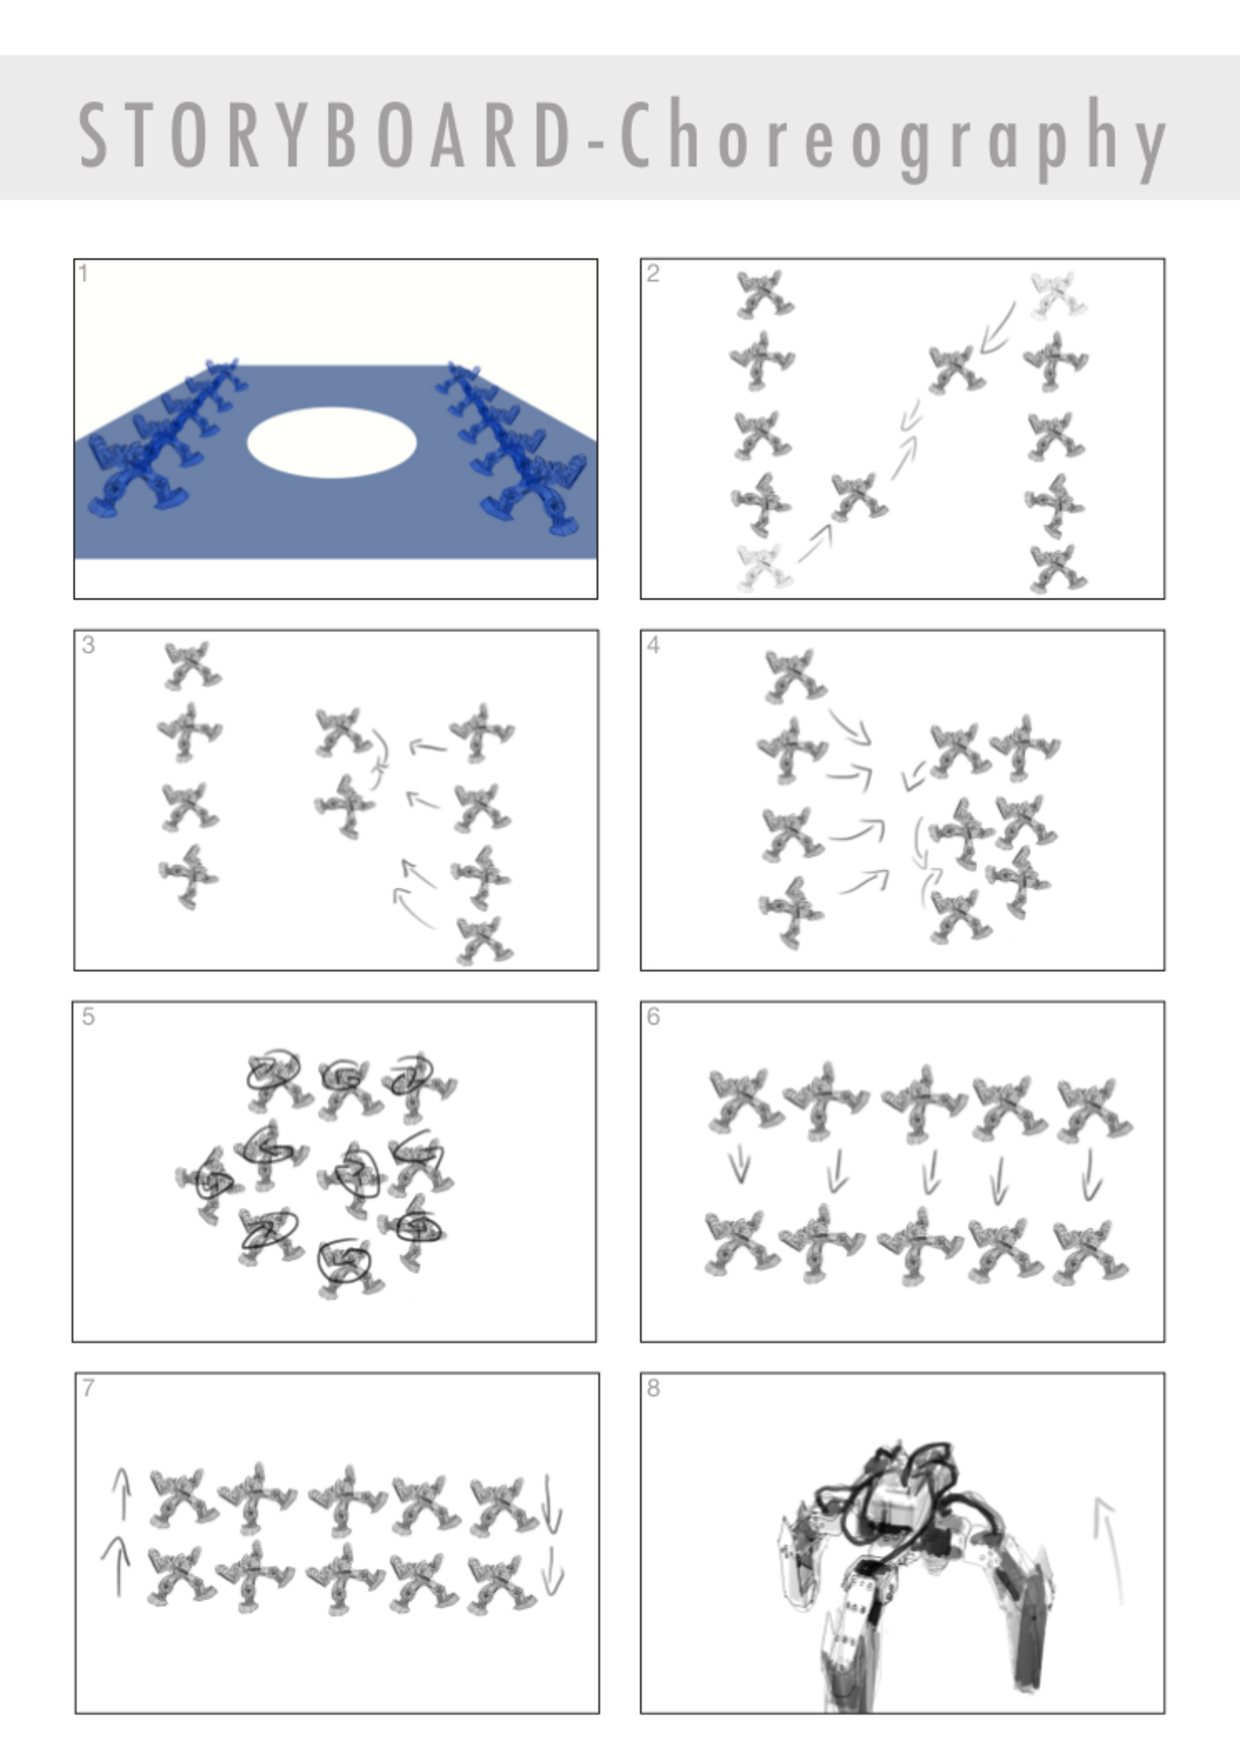
\includepdf[pages={1,2},scale=0.9]{storyboard}
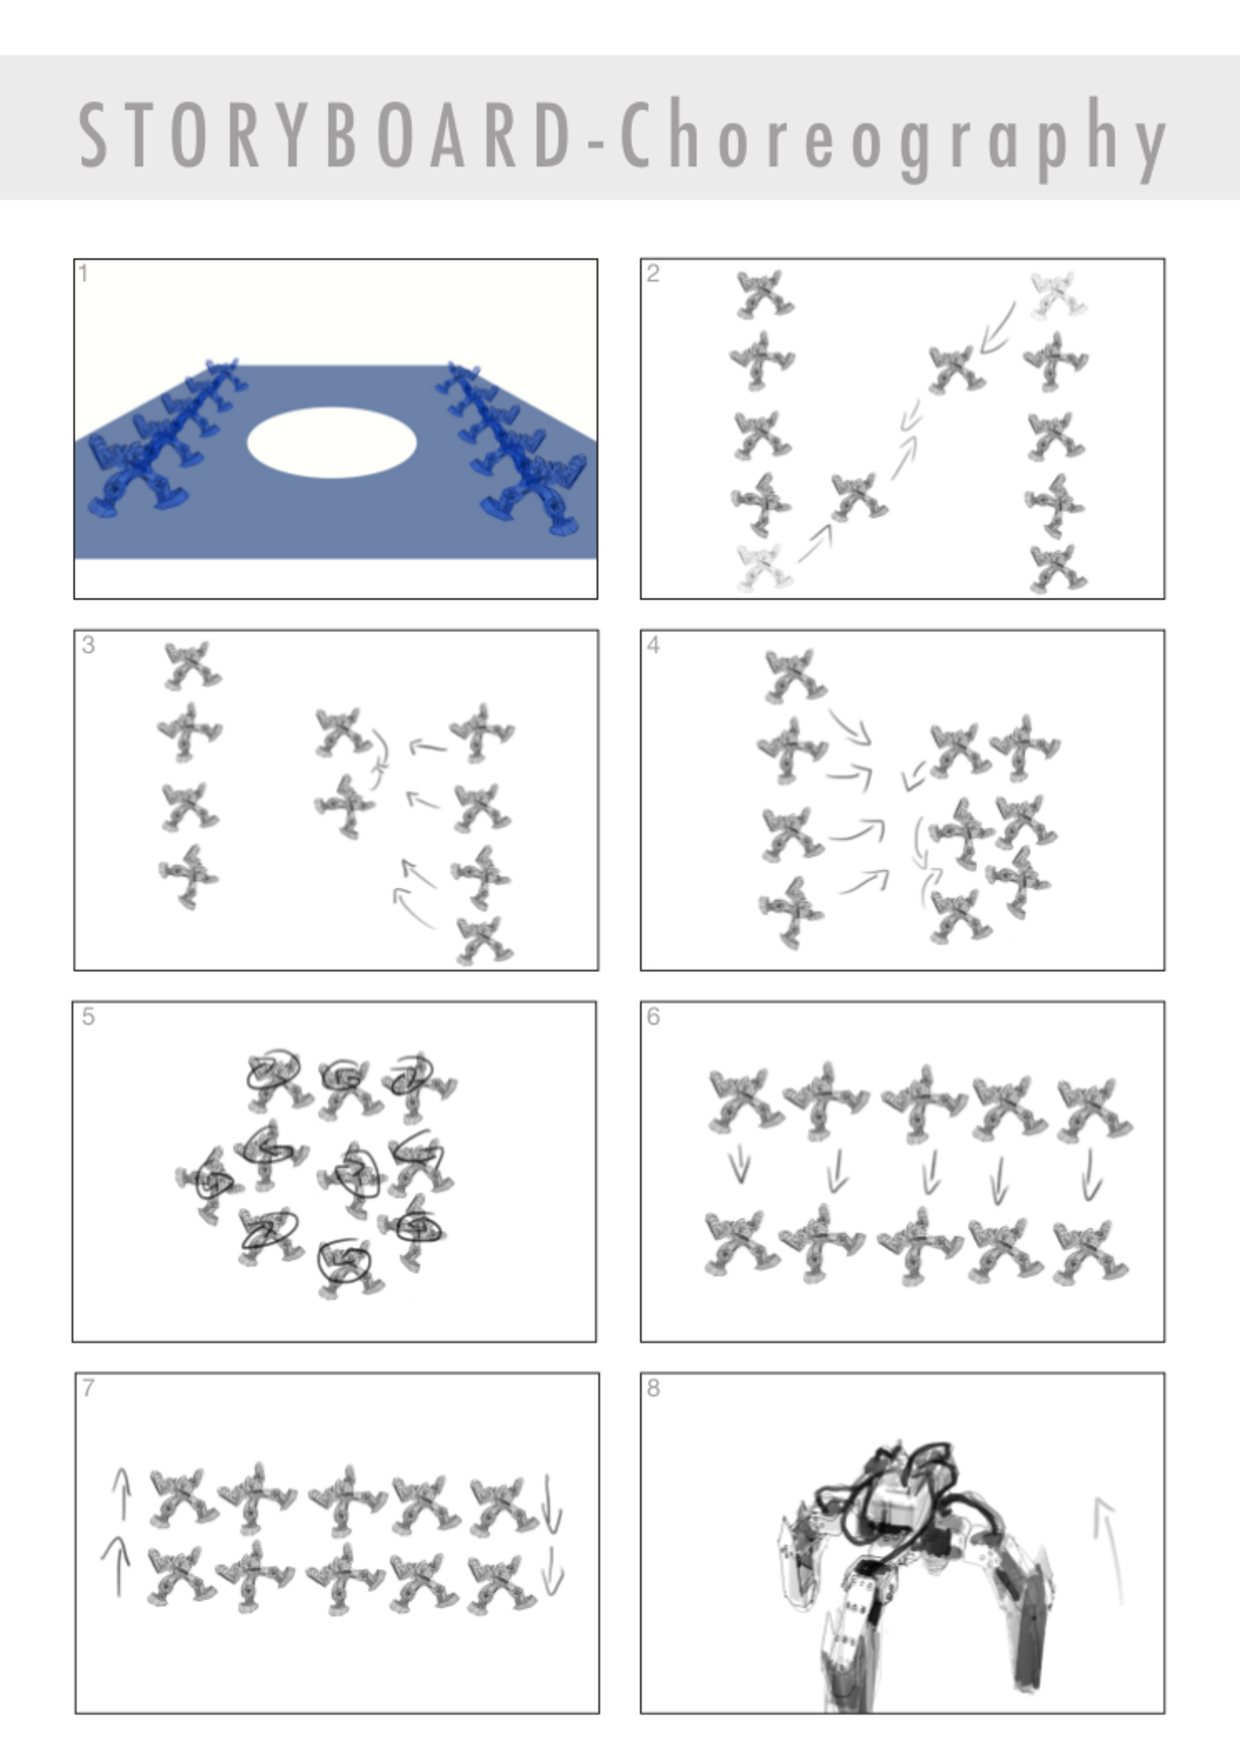
\includepdf[pages={1},scale=0.9]{storyboard}
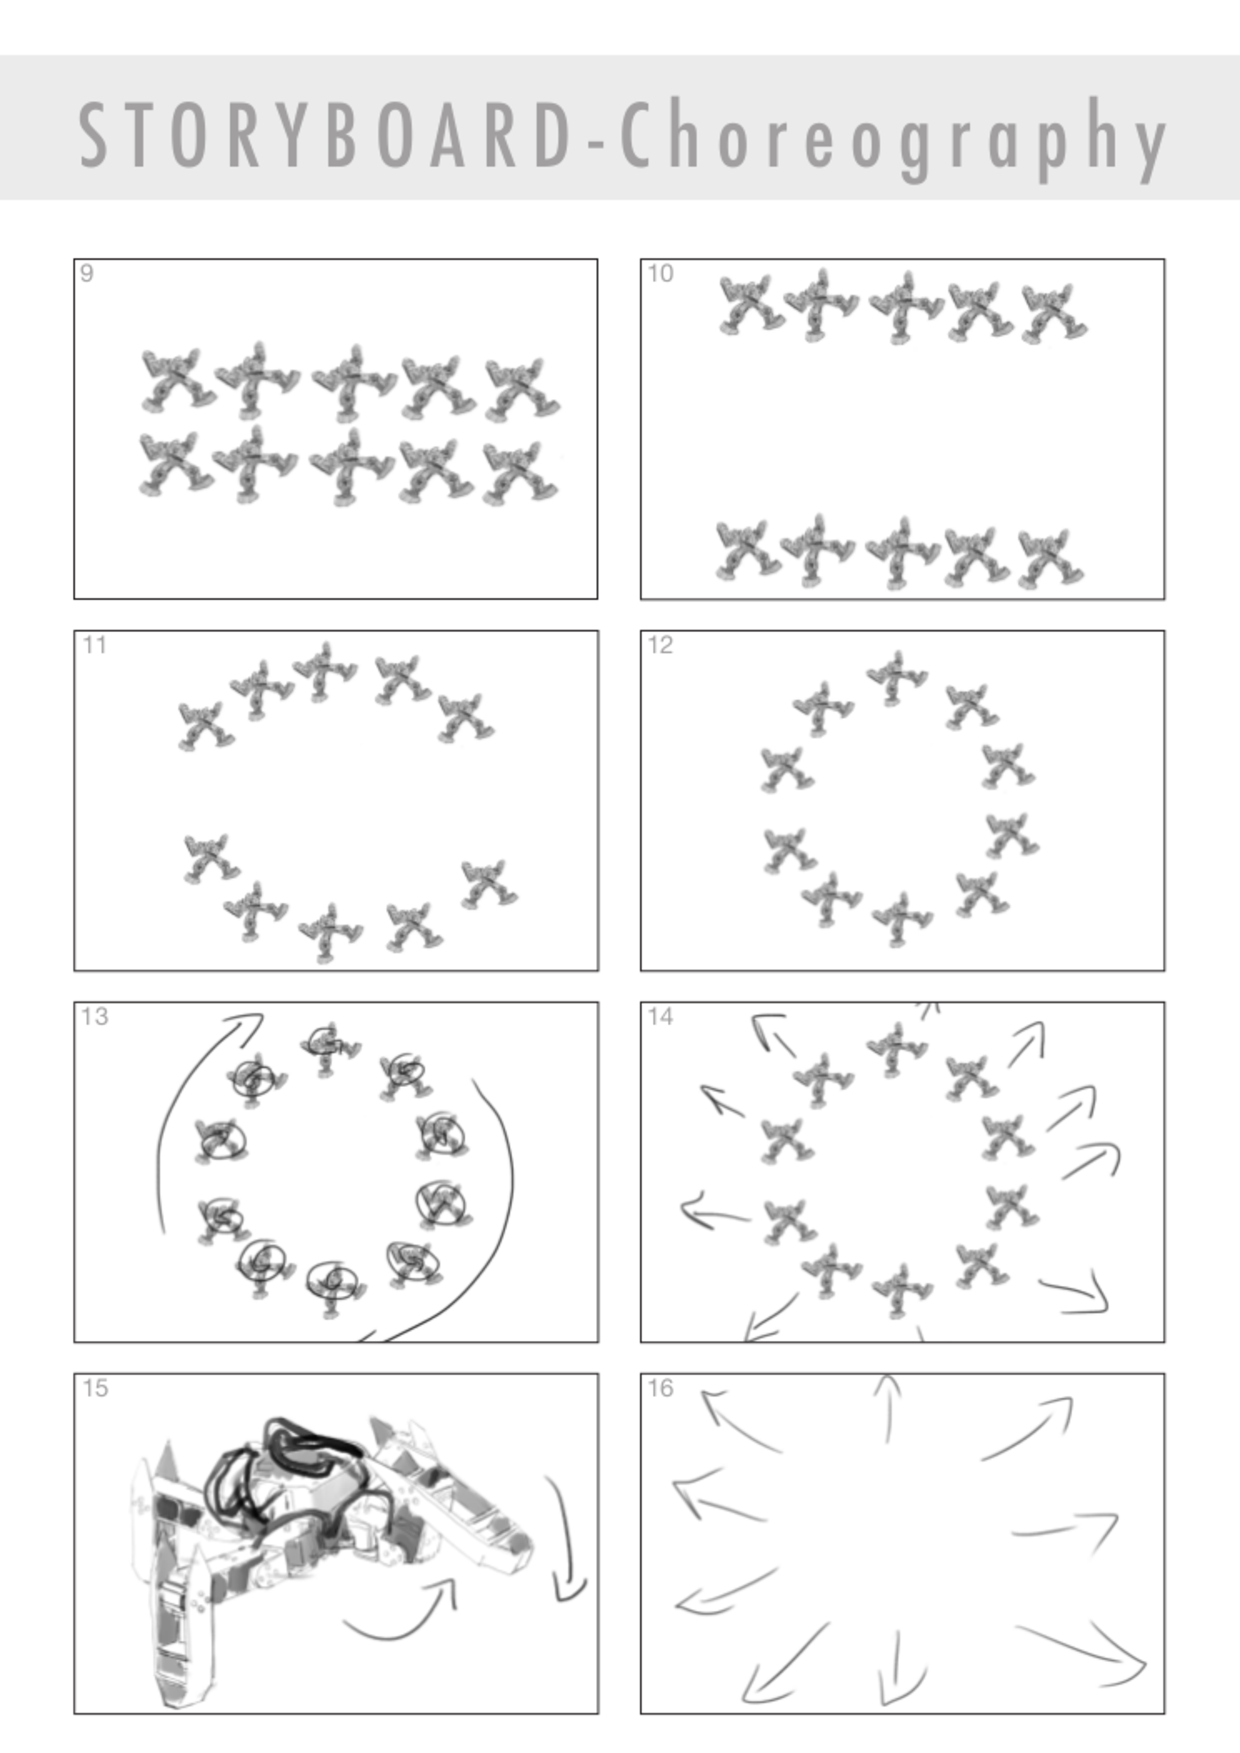
\includepdf[pages={1},scale=0.9]{storyboard2}

%%% End document
\end{document}
